\documentclass[11pt]{beamer}
\usetheme{default}
%\useinnertheme{rounded}

%\useoutertheme[left,hideothersubsections]{IGNsidebar}
\useoutertheme[left,hideothersubsections]{IGNsidebar}




%/usr/share/texmf/tex/latex/beamer/themes/font/beamerfontthemedefault.sty
%/usr/share/texmf/tex/latex/beamer/themes/font/beamerfontthemeprofessionalfonts.sty
%/usr/share/texmf/tex/latex/beamer/themes/font/beamerfontthemeserif.sty
%/usr/share/texmf/tex/latex/beamer/themes/font/beamerfontthemestructurebold.sty
%/usr/share/texmf/tex/latex/beamer/themes/font/beamerfontthemestructureitalicserif.sty
%/usr/share/texmf/tex/latex/beamer/themes/font/beamerfontthemestructuresmallcapsserif.sty
\usefonttheme{structurebold}

\RequirePackage{tikz}

\definecolor{IGNVert}{RGB}{148, 192,  22}
\definecolor{IGNGris}{RGB}{112, 119, 122}

\definecolor{IGNRouge}{RGB}{255, 100, 100}

%PUCES
\setbeamercolor{item projected}{bg=IGNGris!70}

%%%%%%%%%%%%%%%%%%%%%%%%%%%%%%%%%%%%%%%%%%%%%%%%%%% COLOR
\setbeamercolor*{normal text}{fg=IGNGris}

\setbeamercolor{title}{fg=IGNGris}
\setbeamercolor{subtitle}{fg=IGNVert}
\setbeamercolor{item}{fg=IGNVert} 

\setbeamercolor{caption name}{ fg=IGNGris}

%\setbeamercolor{author in head/foot}{ fg=IGNGris}
%\setbeamercolor{institute in head/foot}{fg=IGNGris}
\setbeamercolor{title in head/foot}{ fg=IGNGris}
\setbeamercolor{date in head/foot}{ fg=IGNGris}
\setbeamercolor{page in head/foot}{ fg=IGNGris}
\setbeamercolor{section in toc}{ fg=IGNGris}
\setbeamercolor{subsection in toc}{ fg=IGNGris}

\setbeamercolor*{block title alerted}{bg=IGNRouge!70}
\setbeamercolor*{block body alerted}{bg=IGNRouge!20}

\setbeamercolor*{block title example}{bg=IGNVert!70}
\setbeamercolor*{block body example}{bg=IGNVert!20}

\setbeamercolor*{block title}{bg=IGNGris!50}
\setbeamercolor*{block body}{bg=IGNGris!20}

%%%%%%%%%%%%%%%%%%%%%%%%%%%%%%%%%%%%%%%%%%%%%%%%%%% NAVIGATION SYMBOLS
\setbeamertemplate{navigation symbols}{} 
%%%%%%%%%%%%%%%%%%%%%%%%%%%%%%%%%%%%%%%%%%%%%%%%%%% SIDE BAR
\setbeamersize{sidebar width left=1.5cm}
\setbeamercolor{section in sidebar}{fg=IGNGris}
\setbeamercolor{subsection in sidebar}{fg=IGNGris}

\setbeamercolor{section in sidebar shaded}{fg=IGNVert}
\setbeamercolor{subsection in sidebar shaded}{fg=IGNVert}


\defbeamertemplate*{sidebar}{SSB}{}

%%%%%%%%%%%%%%%%%%%%%%%%%%%%%%%%%%%%%%%%%%%%%%%%%%% HEAD LINE
\defbeamertemplate*{frametitle}{}{
  \begin{tikzpicture}[scale=0.503]
  \filldraw[color=white] (0,0) rectangle(0.1,0.54);
  \end{tikzpicture}
  
    \textcolor{IGNGris}{ \textbf{\insertframetitle}}
  
\begin{tikzpicture}
  \draw[very thick,color=IGNVert] (0,1)--(\paperwidth- 2.24,1);
  \end{tikzpicture} 
}
%%%%%%%%%%%%%%%%%%%%%%%%%%%%%%%%%%%%%%%%%%%%%%%%%%% HEAD LINE
%\defbeamertemplate*{headline}{AH}{
%}

\defbeamertemplate*{headline}{}{}
%%%%%%%%%%%%%%%%%%%%%%%%%%%%%%%%%%%%%%%%%%%%%%%%%%% BACKGROUND

%%%%%%%%%%%%%%%%%%%%%%%%%%%%%%%%%%%%%%%%%%%%%%%%%%% FOOT LINE
\defbeamertemplate*{footline}{}
{
\leavevmode%
  \begin{tikzpicture}
  \draw (0,0) node  {};
  \draw (0.5,0) node[right]  { \textcolor{IGNGris}{\insertshorttitle}};
  \draw (5,0) node[right]  { \textcolor{IGNVert}{$\blacksquare$} \textcolor{IGNGris}{\insertshortdate{} } };
  \draw (7.5,0) node  { \textcolor{IGNVert}{$\blacksquare$} \textcolor{IGNGris}{\insertframenumber{} / \inserttotalframenumber\hspace*{2ex} }};
  %\draw (9.75,0) node  { \textcolor{IGNGris}{ \insertinstitute }};
  \draw (12,0) node[right] { 
\includegraphics[height=0.25cm]{img/LOGO_IGN_p.png} };
  \end{tikzpicture} 

}%


%%%%%%%%%%%%%%%%%%%%%%%%%%%%%%%%%%%%%%%%%%%%%%%%%%% AT BEGIN SECTION


\AtBeginSection[]
{ 
\setbeamercolor{section in sidebar}{fg=white }
\setbeamercolor{subsection in sidebar}{fg=white }

\setbeamercolor{section in sidebar shaded}{fg=white }
\setbeamercolor{subsection in sidebar shaded}{fg=white }



\begin{frame}{
  
\begin{tikzpicture}[scale=0.503]
  \draw[color=IGNGris,fill=IGNGris]  (0,0) rectangle (23,9);
  \draw (1,1) node [right,text width=10cm,text justified]  {  \textcolor{white}{\insertsection}};
  \end{tikzpicture}
}
\end{frame} 


\setbeamercolor{section in sidebar}{fg=IGNGris}
\setbeamercolor{subsection in sidebar}{fg=IGNGris}

\setbeamercolor{section in sidebar shaded}{fg=IGNVert}
\setbeamercolor{subsection in sidebar shaded}{fg=IGNVert}

\addtocounter{framenumber}{-1}

}


\usepackage[english]{babel}
\RequirePackage{tikz}
\usetikzlibrary{arrows}
\usepackage[utf8]{inputenc}
\usepackage{listings}
\usepackage{longtable,booktabs}
%\setbeameroption{show notes}

\def\tightlist{}

%% DONNES UTILES A LA PAGE DE TITRE ET AU PIED DE PAGE...
\graphicspath{{../../images_template/}}

\title[]{MMVII Développement}
\subtitle{IGN - 2024}
%~ \author[shortname]{Jean-Michaël Muller}
%\author[shortname]{Muller J.M. \inst{1} \and Poyard J.C. \inst{1} \and \\Collilieux X. \inst{2}}
%\institute[shortinst]{\inst{1} IGN SGN, Saint-Mandé, France \and %
%                      \inst{2} IGN LAREG, Université Paris Diderot - Sorbonne Paris Cité, Paris, France}
\date{CM}

\newenvironment{smallverbatim}%
  {\verbatim\small}%
  {\endverbatim}


\begin{document}


\usebackgroundtemplate{
        \begin{tikzpicture}
        %\draw (0,0.5) node[right] { 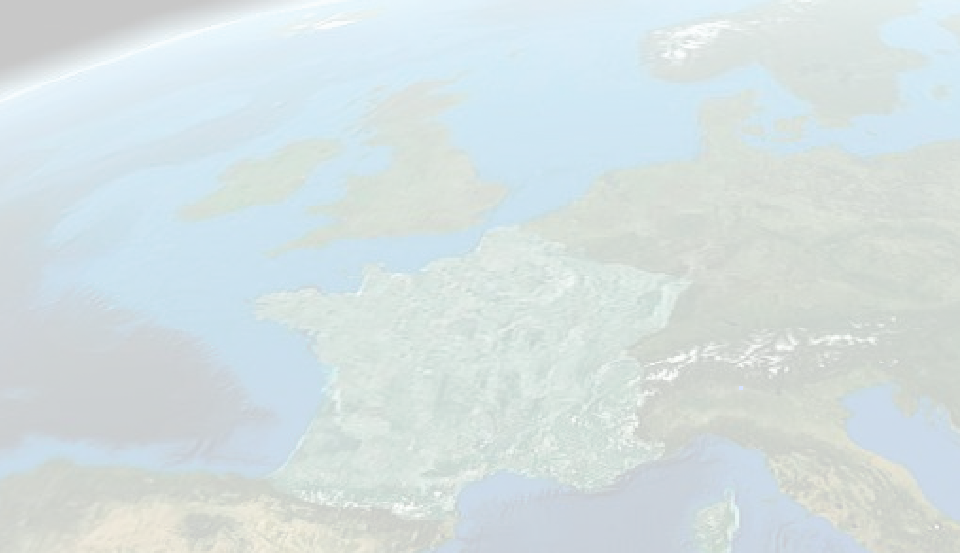
\includegraphics[width=12.5cm]{img/fondClair.png} };
        \draw (0,5) node[right] { 
\includegraphics[height=1.5cm]{img/LOGO_IGN2.png} };
        %\draw (4,5) node[right] { \includegraphics[height=1.5cm]{img/hrao.png} };
        %\draw (11,5) node[right] { \includegraphics[height=1.5cm]{img/IAG.png} };
        %\draw (7.2,5) node[right] { \includegraphics[height=1.5cm]{img/logoISPRS2016.png} };
        %\draw (11,5) node[right] { \includegraphics[height=1.5cm]{img/LOGO_MATIS.png} };
%        \draw (1.5,4.95) node[right] { \includegraphics[width=3.5cm]{fondD.jpg} };
        \end{tikzpicture}   
}

\begin{frame}[plain,c]
\begin{columns}
\begin{column}{10cm}
\begin{center}
\vspace{2cm}
{
%\tiny, \scriptsize, \footnotesize, \small, \normalsize, \large, \Large, \LARGE, \huge, \Huge.
\LARGE
\usebeamerfont{title}\usebeamercolor[fg]{title}\inserttitle}

\vspace{0.3cm}

{\small \insertsubtitle}

\vspace{0.3cm}

\normalsize

\insertauthor



\normalsize
\vspace{0.5cm}

\insertinstitute


\vspace{0.5cm}

\insertdate


\end{center}
\end{column}
\begin{column}{1cm}
\end{column}
\end{columns}

\end{frame}



%%%%%%%%%%%%%%%%%%%%%%%%%%%%%%%%%%%%%%%%%%%%%%%%%%%%%%%%%%%%%%%%%%%%%%%%%%%%%%%%%%%%%%%%%%%%%%%%%%%%%%%%%
% DEBUT DE LA PRESENTATION
% BACKGROUND POUR AVOIR LE HAUT DE PAGE QUI VA BIEN
\usebackgroundtemplate{
    
\begin{tikzpicture}[scale=0.503]
    \filldraw[color=IGNGris] (0,0) rectangle(2.62,0.54);
    \filldraw[color=IGNGris] (4.77,0) rectangle(2.62+4.77,0.54);
    
    \filldraw[color=IGNVert] (9.50+0.27,0) -- (9.50,0.54)-- (9.50+7.41-0.27,0.54)-- (9.50+7.41,0)--cycle;
    
    \filldraw[color=IGNGris] (19.50,0) rectangle(2.62+19.50,0.54);
    \filldraw[color=IGNGris] (23.11,0.54)--(23.11+0.54,0)--(2.3+23.11,0)--(2.3+23.11,0.54)--cycle;;
    \end{tikzpicture}   
}


%%%%%%%%%%%%%%%%%%%%%%%%%%%%%%%%%%%%%%%%%%%%%%%%%%%%%%%%%%%%%%%%%%%%%%%%%%%%%%%%%%%%%%%%%%%%%%%%%%%%%%%%%
% PLAN
\setbeamercolor{section in sidebar}{fg=white } %LIGNE NECESSAIRE POUR EFFACER LE PLAN DE LA SIDEBAR (PAS MIEUX)
\setbeamercolor{subsection in sidebar}{fg=white }%LIGNE NECESSAIRE POUR EFFACER LE PLAN DE LA SIDEBAR (PAS MIEUX)
\setbeamercolor{section in sidebar shaded}{fg=white }%LIGNE NECESSAIRE POUR EFFACER LE PLAN DE LA SIDEBAR (PAS MIEUX)
\setbeamercolor{subsection in sidebar shaded}{fg=white }%LIGNE NECESSAIRE POUR EFFACER LE PLAN DE LA SIDEBAR (PAS MIEUX)
\begin{frame}
  \begin{columns}[T]
  \begin{column}{7cm}
  \tableofcontents[sections={1-5},hideallsubsections]
  \end{column}
  %\begin{column}{5cm}
  %\tableofcontents[sections={6-10},hideallsubsections]
  %\end{column}
  \end{columns}

\end{frame}
\setbeamercolor{section in sidebar}{fg=IGNGris}%LIGNE NECESSAIRE POUR AFFICHER LE PLAN DE LA SIDEBAR (PAS MIEUX)
\setbeamercolor{subsection in sidebar}{fg=IGNGris}%LIGNE NECESSAIRE POUR AFFICHER LE PLAN DE LA SIDEBAR (PAS MIEUX)
\setbeamercolor{section in sidebar shaded}{fg=IGNVert}%LIGNE NECESSAIRE POUR AFFICHER LE PLAN DE LA SIDEBAR (PAS MIEUX)
\setbeamercolor{subsection in sidebar shaded}{fg=IGNVert}%LIGNE NECESSAIRE POUR AFFICHER LE PLAN DE LA SIDEBAR (PAS MIEUX)




%%%%%%%%%%%%%%%%%%%%%%%%%%%%%%%%%%%%%%%%%%%%%%%%%%%%%%%%%%%%%%%%%%%%%%%%%%%%%%%%%%%%%%%%%%%%%%%%%%%%%%%%%
\input{"presentation.tex"}
%%%%%%%%%%%%%%%%%%%%%%%%%%%%%%%%%%%%%%%%%%%%%%%%%%%%%%%%%%%%%%%%%%%%%%%%%%%%%%%%%%%%%%%%%%%%%%%%%%%%%%%%%

\end{document}
